\RequirePackage{shellesc}
\immediate\write18{cd ..; tex spath3_code.dtx}
\documentclass{article}

\usepackage{tikz}
\usetikzlibrary{spath3,intersections}

\begin{document}

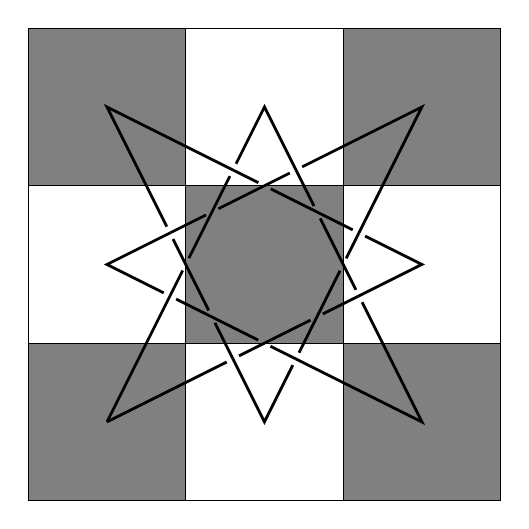
\begin{tikzpicture}

\fill[gray]
(0,0) rectangle +(2,2)
(2,2) rectangle +(2,2)
(4,4) rectangle +(2,2)
(0,4) rectangle +(2,2)
(4,0) rectangle +(2,2)
;
\draw (0,0) grid[step=2] (6,6);

\path[
  spath/save=tour,
  line width=1pt,
]
(1,1)
-- ++(4,2)
-- ++(-4,2)
-- ++(2,-4)
-- ++(2,4)
-- ++(-4,-2)
-- ++(4,-2)
-- ++(-2,4)
-- ++(-2,-4)
;

\tikzset{
  spath/.cd,
  split at self intersections=tour,
  remove empty components=tour,
  insert gaps after components={tour}{5pt}{1,3,...,31},
  spot weld,
  get components of={tour}\pathcomponents,
}

\foreach[count=\k] \cpt in \pathcomponents {
   \draw[line width=1pt,spath/restore=\cpt];
%  \node[fill=white, fill opacity=.5, circle, text opacity=1] at (spath cs:{\cpt} .5) {\(\k\)};
}

\end{tikzpicture}

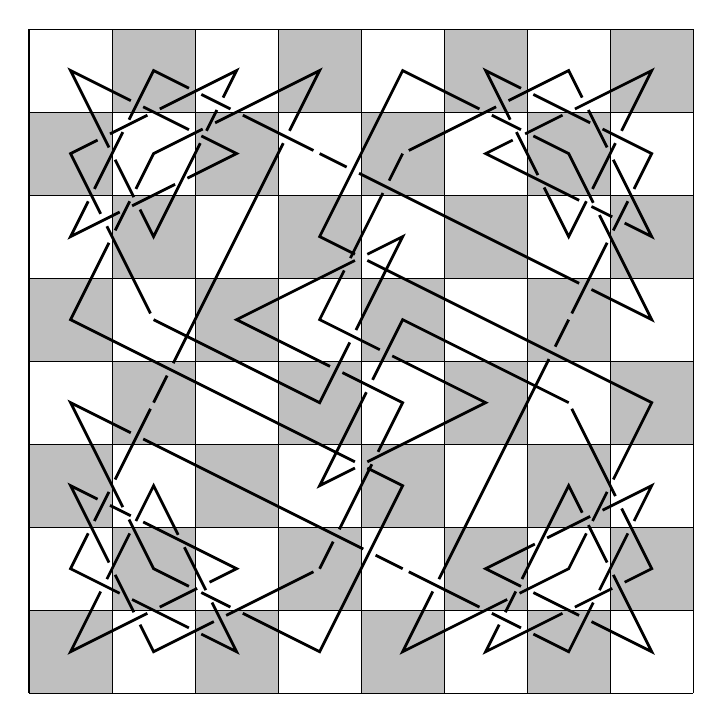
\begin{tikzpicture}[
  x={(30pt,0pt)},
  y={(0pt,30pt)}
]

\foreach \x in {0,1,...,7}
{
\foreach[evaluate=\y as \xy using {int(mod(\x+\y,2))}] \y in {0,1,...,7}
  {
    \ifnum\xy=0\relax
    \fill[gray!50!white] (\x-4,\y-4) rectangle +(1,1);
    \fi
  }
}
\draw (-4,-4) grid[step=1] +(8,8);

\path[
%  draw,
  gray!50!white,
  line width=3pt
]
(-4,-4)
++(.5,.5)
-- ++(2,1)
-- ++(-2,1)
-- ++(1,-2)
-- ++(2,1)
-- ++(1,2)
-- ++(-2,1)
-- ++(2,1)
-- ++(-1,-2)
-- ++(-2,1)
-- ++(-1,2)
-- ++(2,1)
-- ++(-1,-2)
-- ++(-1,2)
-- ++(2,-1)
-- ++(-2,-1)
-- ++(1,2)
-- ++(2,-1)
-- ++(2,-1)
-- ++(2,-1)
-- ++(-1,2)
-- ++(-2,1)
-- ++(-1,-2)
-- ++(2,-1)
-- ++(2,-1)
-- ++(-1,-2)
-- ++(-2,-1)
-- ++(1,2)
-- ++(1,2)
-- ++(1,2)
-- ++(-2,1)
-- ++(1,-2)
-- ++(1,2)
-- ++(-2,-1)
-- ++(2,-1)
-- ++(-1,2)
-- ++(-2,-1)
-- ++(-1,-2)
-- ++(2,-1)
-- ++(-2,-1)
-- ++(1,2)
-- ++(2,-1)
-- ++(1,-2)
-- ++(-2,-1)
-- ++(1,2)
-- ++(1,-2)
-- ++(-2,1)
-- ++(2,1)
-- ++(-1,-2)
-- ++(-2,1)
-- ++(-2,1)
-- ++(-2,1)
-- ++(1,-2)
-- ++(2,-1)
-- ++(1,2)
-- ++(-2,1)
-- ++(-2,1)
-- ++(1,2)
-- ++(2,1)
-- ++(-1,-2)
-- ++(-1,-2)
-- ++(-1,-2)
-- ++(2,-1)
-- ++(-1,2)
%-- ++(-1,-2)
-- cycle
;

\path[
  spath/save=corner,
%  draw
]
(-4,-4)
++(1.5,3.5)
-- ++(-1,-2)
-- ++(2,-1)
-- ++(-1,2)
-- ++(-1,-2)
-- ++(2,1)
-- ++(-2,1)
-- ++(1,-2)
-- ++(2,1)
%-- ++(1,2)
;

\path[
  spath/save=centre,
%  draw
]
(-4,-4)
++(4.5,1.5)
-- ++(-2,1)
-- ++(-2,1)
-- ++(1,-2)
-- ++(2,-1)
-- ++(1,2)
%-- ++(-2,1)
%-- ++(-2,1)
;

\path[
  spath/save=triangle,
%  draw,
  rotate=180
]
(-4,-4)
++(3.5,1.5)
-- ++(1,2)
-- ++(-2,1)
-- ++(2,1)
-- ++(-1,-2)
;

\path[
  spath/save=centre line
]
(.5,-1.5)
-- ++(-2,1)
;

\path[
  spath/save=edge line
]
(-.5,-2.5)
-- ++(1,2)
;

\tikzset{
%  remove empty components=corner,
%  remove empty components=centre,
%  remove empty components=triangle,
  %
  spath/.cd,
  transform={corner}{scale=.5},
  transform={centre}{scale=.5},
  transform={triangle}{scale=.5},
  transform={centre line}{scale=.5},
  %
  clone={centre line 180}{centre line},
  transform={centre line 180}{rotate=180},
  %
  split at self intersections=corner,
  split at self intersections=centre,
  split at self intersections=triangle,
  %
  split at intersections={triangle}{centre line 180},
  split at intersections={triangle}{centre line},
  %
  clone={triangle 180}{triangle},
  transform={triangle 180}{rotate=180},
  %
  split at intersections={corner}{centre},
  split at intersections={centre}{triangle 180},
  split at intersections={triangle}{triangle 180},
  %
  transform={corner}{scale=2},
  transform={centre}{scale=2},
  transform={triangle}{scale=2},
  transform={triangle 180}{scale=2},
  transform={centre line}{scale=2},
  transform={centre line 180}{scale=2},
  %
  insert gaps after components={corner}{5pt}{1,3,...,33},
  insert gaps after components={centre}{5pt}{2,4,...,10},
  insert gaps after components={triangle}{5pt}{1,3,...,11},
  insert gaps after components={triangle 180}{5pt}{2,4,...,10},
  insert gaps after components={centre line}{5pt}{1},
  %
  clone={tour}{corner},
  clone={centre reversed}{centre},
  %
  transform={edge line}{rotate=-90},
  transform={corner}{rotate=-90},
  transform={centre}{rotate=180},
  transform={centre line}{rotate=180},
  transform={centre reversed}{rotate=90},
  %
  reverse=centre reversed,
  reverse=corner,
  reverse=edge line,
%
  join with={tour}{triangle 180},
  join with={tour}{edge line},
  join with={tour}{corner},
  join with={tour}{centre},
  join with={tour}{centre line},
  join with={tour}{centre reversed},
%
  clone={tour 180}{tour},
  transform={tour 180}{rotate=180},
%
  join with={tour}{tour 180},
  spot weld={tour},
  export to svg={tour}
%  show spath={tour},
}

\draw[line width=1pt, spath/restore=tour];
\end{tikzpicture}
\end{document}
